
% PREAMBULO DO DOCUMENTO
\documentclass[12pt,a4paper,oneside]{book}                      % tipo de documento
\usepackage[top=3cm,bottom=2cm,right=2cm,left=3cm]{geometry}    % margem
\usepackage[utf8x]{inputenc}                                    % acentuacao
\usepackage{ucs}
%\usepackage[light,math]{anttor} 								% fonte. http://www.tug.dk/FontCatalogue/
\usepackage[T1]{fontenc}
\usepackage[brazil]{babel}                                      % hifenizacao
\usepackage{amsmath}                                            % pacote matemática
\usepackage{indentfirst} 										% identacao dos paragrafos
\usepackage{hyperref} 											% hiperlinks (itens clicaveis)
\usepackage{graphicx} 											% ferramentas graficas
\usepackage{amsmath} 											% ferramentas matematicas
\usepackage{amsfonts}											% ferramentas matematicas
\usepackage{amssymb}											% ferramentas matematicas
\usepackage{pdfpages}											% inclusao de paginas em pdf
\usepackage{epstopdf}											% inclusao de figuras em eps
\usepackage{xcolor}												% habilita cores (capa)
\usepackage[some]{background} 									% papel de parede (capa)
\usepackage{color,soul} %para marcação em amarelo do texto
\usepackage[titletoc]{appendix} %para apêndices
\renewcommand\appendixtocname{Apêndices}
\usepackage{longtable} %para tabelas que ultrapassam uma página
\usepackage{framed} %para caixas ao redor do texto


% CONFIGURACAO DA CAPA
%
\definecolor{titlepagecolor}{cmyk}{0.10,.05,.05,.3} % definicao de cor

\backgroundsetup{
scale=1,
angle=0,
opacity=1,
contents={\begin{tikzpicture}[remember picture,overlay]
 \path [fill=titlepagecolor] (current page.west)rectangle (current page.north east); 
 %\draw [color=white, very thick] (5,0)--(5,0.5\paperheight);
\end{tikzpicture}}
} % configura o plano de fundo






\makeatletter                   
\def\printauthor{%                  
    {\large \@author}}          
\makeatother
% FIM DA CONFIGURACAO DA CAPA

\title{Índice de Governança Corporativa}% titulo do documento
\date{Dezembro de 2020}% (sem) data

\author{Dezembro de 2020}

% INICIO DO DOCUMENTO
%
\begin{document}
%
% CONSTRUCAO DA CAPA
%
\begin{titlepage}
\BgThispage
\newgeometry{left=1cm,right=2cm,bottom=2cm}
\vspace*{0.30\textheight}
\noindent
\begin{center}
\textcolor{black}{{\Huge\textbf{Índice de Governança Corporativa}}\\ 
\vspace{20pt}}
\Large\textbf{Perspectiva I - Conformidade Legal e Boas Práticas}
\end{center}



\vspace{40pt}

\large{    
Diretoria Central de Governança das Estatais
    
Superintendência Central de Governança de Ativos e da Dívida Pública
    
Subsecretaria do Tesouro Estadual - SEF/MG}
    
\vspace{40pt}
    
Janeiro, 2021

\begin{figure}[b]    
\begin{flushright}

\includegraphics[width=60mm]{figures/logo-tesouro-peq.png}
\end{flushright}
\end{figure}
	
\end{titlepage}
\restoregeometry
%
% FIM DA CONSTRUCAO DA CAAPA
	
%----------------------------
\tableofcontents % sumario
\clearpage
%----------------------------
	
\chapter*{Prefácio}
\addcontentsline{toc}{chapter}{Preâmbulo}

\hl{Inserir algum texto introdutorio, pode ser uma declaracao do Ramon, Andresa ou do Subsecretario}
	
	
\chapter{Introdução}
\label{chp:intro}
	
\section{Objetivo}
	
O principal objetivo do Índice de Governança Corporativa elaborado pela Diretoria Central de Governança das Estatais - DCGE é aferir o aderência da governança corporativa das estatais mineiras aos dispositivos legais pertinentes, quais sejam a Lei 13.303, de 30 de junho de 2016 (Lei das Estatais), do Decreto 47.154, de 20 de fevereiro de 2017 e Decreto Estadual 47,105, de 16 de dezembro de 2016, e às boas práticas recomendadas pela OCDE - Organização para Cooperação e Desenvolvimento Econômico, em especial aquelas abordadas em duas publicações:"Diretrizes da OCDE sobre Governança Coporativa de Empresas Estatais" e \textit{"Accountability and Transparency - A guide for state ownership"}.
	
As diretrizes da OCDE constituem relevante referência pois consolidam "recomendações aos governos sobre como assegurar que as empresas estatais operem de forma eficiente, transparente e responsável" sendo "o padrão internacionalmente aceito sobre a maneira como os governos devem exercer a função de propriedade estatal para evitar armadilhas da titularidade passiva e da intervenção estatal" \citep[p.~7]{ocde-diretrizes}. 
	
Nesse sentido, ressalte-se que a própria elaboração de um índice de governança corporativa representa a materialização de um das boas práticas sumarizadas pela OCDE. A fim de se constituir um Estado Acionista informato e ativo, consta dentre as recomendações a "criação de sistemas de relatoria que permitam que a entidade proprietária acompanhe, audite e avalie regularmente o desempenho das empresas estatais e, supervisão e monitoramento da sua conformidade com os padrões aplicáveis de governança corporativa".\citep[p.~21]{ocde-diretrizes}

Cabe pontuar que a aferição do índice não apresenta caráter punitivo, sendo sua função meramente informativa. Desse modo, espera-se que tanto a Diretoria Central de Gestão das Estatais quanto as próprias empresas possam munir-se das informações resultantes do diagnóstico para identificados os pontos de melhoria que demandam atenção e promover melhorias na governança corporativa. 
	
Dessa forma, a execução de rodadas consecutivas de avaliação do índice possibilitará em médio e longo prazo a criação de um panorama evolutivo da maturidade e eficiência das estatais mineiras.
	
%\section{Alinhamento com o IG-SEST}
	
%Sempre que possível, foi mantido o alinhamento com o IG - SEST, o Indicador de Governança da Secretaria de Coordenação de Governança das Empresas Estatais.
	
\section{Perspectivas e Dimensões de Análise}
	
Propõe-se a análise de um Índice de Governança Corporativa  aferido em três perspectivas de análise:
	
\begin{itemize}
	\item \textbf{Perspectiva I} - Análise de conformidade legal e aderência às boas práticas recomendadas pela OCDE. Esta é a perspectiva abordada neste volume, que abordará as dimensões de critérios legais básicos, práticas de gestão, controle interno e gestão de riscos, transparência e atendimento à DCGE. Esta aferição guarda bastante similaridade ao IG-SEST, o Indicador de Governança  da Secretaria de Coordenação e Governança das Empresas Estatais, do Ministério da Economia.
		
	\item \textbf{Perspectiva II} - Análise de eficiência numa perspectiva comparativa interna ao cenário mineiro. \hl{COMENTAR}
		
	\item \textbf{Perspectiva III} - Análise de eficiência dentro do setor. Perspectiva comparativa no cenário nacional. Análise econométrica para construção da curva de eficiência. \hl{COMENTAR}
	\end{itemize}

%\subsection{Perspectiva I}
%Para a primeira aferição do índice, as análise estará restrita à primeira perspectiva, que estará estruturada nas seguintes dimensões: critérios legais básicos, práticas de gestão, controle interno e gestão de riscos, transparência e atendimento à DCGE.

%\subsection{Perspectiva II}

%\subsection{Perspectiva III}
	
\section{Escopo}
	
Nesta análise serão objeto de avaliação as empresas estatais dependentes e 
\hl{falar das empresas que farao parte das analises}
	
\chapter{Metodologia e Operacionalização}
\label{chp:metodologia}
	
\section{Comissão de Avaliação}
\label{sec:comissao}

\section{Indicação de responsáveis pelas informações prestadas}
    
\hl{ver se houve formalizacao para designacao dos interlocutores das estatais}
	
\section{Calendário}
\label{sec:calendario}

Descrever processo de avaliação (ex: Durante o primeiro trimestre do ano a comissão de avaliação designada..... A frequência de apuração será anual?)

\hl{IG-SEST pag. 4 A frequencia de apuracao do IG e semestral e sera gerado um relatorio de avaliacao para cada empresa participante contendo analises das informacoes e evidencias fornecidas pelas empresas, relatando a evolucao do nivel de governanca, cujos resultados se restringem ao uso reservado e exclusivo da estatal.}
	
\section{Formulários}
\hl{Descrever como serão disponibilizados os formularios. Ver criterios tecnicos com Pedro e Eduardo}


\section{Forma de Cálculo}

Recebidas as informações das estatais, será realizada a apuradas pela Comissão de Avaliação designada conforme apresentado no item \ref{sec:comissao}. 

A nota final do Índice de Governança Corporativa será calculada conforme se apresenta a seguir. Às dimensões de análise serão dados os pesos conforme mostrado na Figura \ref{fig:pesos-dimensoes}.

\begin{figure}[h]
\label{fig:pesos-dimensoes}
\caption{Pesos das Dimensões de Análise}
\centering
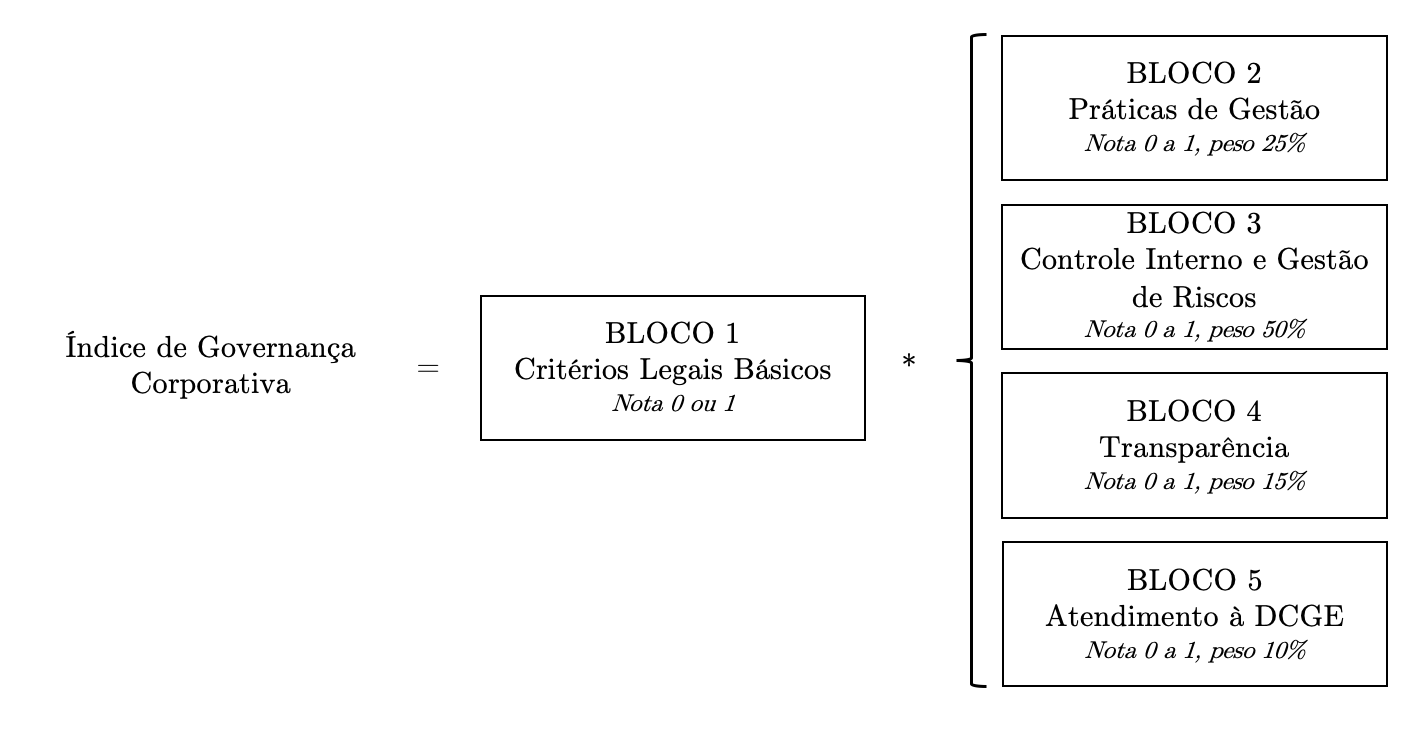
\includegraphics[width=\textwidth]{figures/ig-perspectiva1.png}
\end{figure}

Para as dimensões "Práticas de Gestão", "Controle Interno e Gestão de Risco", "Transparência" e "Atendimento à DCGE" serão computadas uma nota entre 0 e 1. Para a dimensão "Critérios Legais Básicos" a nota será 0 ou 1, isso porque esta dimensão assumirá o papel de um mecanismo "passa ou falha". Ou seja, caso a nota final dessa dimensão seja 1, a nota final do indicador será aquela computada de acordo com o peso das demais dimensões, porém, caso a nota seja 0, as demais notas serão zeradas. Esse mecanismo foi adotado para refletir a hierarquia das prioridades já que na dimensão "Critérios Legais Básicos" são tratados aspectos legais centrais e basilares.

Com relação à distribuição de pesos, para a dimensão "Práticas de Gestão" o peso da nota será de 25\%, para a dimensão "Controle Interno e Gestão de Risco" o peso será de 50\%, para a dimensão "Transparência" o peso será de 15\% e para a dimensão "Atendimento à DCGE" o peso será de 10\%, também conforme apresentado na Figura \ref{fig:pesos-dimensoes}.

Dessa forma, a fórmula de cômputo do Índice de Governança Corporativa - IGC é:

\begin{equation}
IGC = \text{Bloco 1} \times \frac{\sum{\text{Peso Bloco}_i * \text{Nota Bloco}_i}}{\sum{\text{Peso Bloco}_i}}
\end{equation}

na qual, 

\({IGC}\) é o Índice de Governança Corporativa

\({i}\) são os blocos 2 a 5, quais sejam Bloco 2 - Práticas de Gestão, Bloco 3 - Controle Interno e Gestão de Riscos, Bloco 4 - Transparência e Bloco 5 - Atendimento à DCGE

Relativamente ao cômputo das notas dos blocos, aplica-se a seguinte regra:

\begin{itemize}

    \item Para o Bloco 1, a nota final será 1 apenas no caso em que a totalidade das questões retorne valor 1. Caso contrário, será aplicado nota 0.
    
    \item Para os Blocos 2 a 5, as notas serão o somatório das respostas atribuídas às respectivas questões, sendo assumido peso igual entre as questões dentro do mesmo bloco.
    
\end{itemize}

\chapter{Produtos e Resultados}
	
\hl{ver com pedro sobre painel informacoes para publicacao dos resultados do indicador. Ver formularios sharepoint para coleta de informacoes. Ver acesso externo para interlocutores preencherem sharepoint. Fazer relatorio de cada empresa como o IG-SEST faz???}

\phantomsection
\addcontentsline{toc}{chapter}{Bibliografia}
\bibliography{referencias}
\bibliographystyle{siam} % siam abbrv amsplain plain  

\begin{appendices}
\chapter{Questionários}
\label{chp:quest}

%Bloco 1
\begin{center}
\begin{longtable}{c l c c}
\caption{Bloco 1 - Critérios Legais Básicos} \label{tab:dim_zero} \\
\hline
 Item & Pergunta & Referência & Respostas \\ 
 \hline
1.1  & \parbox[t]{8cm}{O estatuto da companhia respeita a composição do Conselho de Administração com mínimo de 7 (sete) e máximo de 11 (onze) membros, ou outra instituída pela lei que autorizou a criação da empresa?} & \parbox[t]{2cm}{Lei 13.303,\\ art. 13, I} & \parbox[t]{2cm}{$\square$ Sim (1) \\ $\square$ Não (0)}\\  
1.2 &\parbox[t]{8cm}{O estatuto da companhia respeita a composição mínima da Diretoria Executiva de 3 diretores?} & \parbox[t]{2cm}{Lei 13.303, art. 13, II} & \parbox[t]{2cm}{$\square$ Sim (1) \\ $\square$ Não (0)}\\ 
1.3 &\parbox[t]{8cm}{O estatuto da companhia respeita o limite legal definido para o prazo de gestão dos administradores  como não superior a 2 anos?} & \parbox[t]{2cm}{Lei 13.303, art. 13, VI} & \parbox[t]{2cm}{$\square$ Sim (1) \\ $\square$ Não (0)}\\
1.4 &\parbox[t]{8cm}{O estatuto da companhia respeita o limite legal máximo de 3 reconduções consecutivas para os administradores?} & \parbox[t]{2cm}{Lei 13.303, art. 13, VI} & \parbox[t]{2cm}{$\square$ Sim (1) \\ $\square$ Não (0)}\\ 
1.5 &\parbox[t]{8cm}{O estatuto da companhia prevê a participação de representante dos empregados no Conselho de Administração?} & \parbox[t]{2cm}{Lei 13.303, art. 13, VI} & \parbox[t]{2cm}{$\square$ Sim (1) \\ $\square$ Não (0)}\\ 
1.6 &\parbox[t]{8cm}{O estatuto da companhia prevê a representação mínima legal de 25\% de membros independentes ou por pelo menos 1 (um), caso haja decisão pelo exercício da faculdade do voto múltiplo pelos acionistas minoritários, nos termos do art. 141 da Lei nº 6.404, de 15 de dezembro de 1976?} & \parbox[t]{2cm}{Lei 13.303, art. 13, VI} & \parbox[t]{2cm}{$\square$ Sim (1) \\ $\square$ Não (0)}\\ 
1.7 &\parbox[t]{8cm}{O estatuto da empresa prevê requisitos específicos para o exercício do cargo de diretor?} & \parbox[t]{2cm}{Lei 13.303, art. 13, II} & \parbox[t]{2cm}{$\square$ Sim (1) \\ $\square$ Não (0)}\\
1.8 &\parbox[t]{8cm}{O estatuto da empresa prevê avaliação de desempenho, individual e coletiva, de periodicidade anual, dos administradores e dos membros de comitês?} & \parbox[t]{2cm}{Lei 13.303, art. 13, III} & \parbox[t]{2cm}{$\square$ Sim (1) \\ $\square$ Não (0)}\\
1.9 &\parbox[t]{8cm}{O estatuto da companhia prevê a constituição e funcionamento do Conselho Fiscal?} & \parbox[t]{2cm}{Lei 13.303, art. 13, IV} & \parbox[t]{2cm}{$\square$ Sim (1) \\ $\square$ Não (0)}\\
1.10 &\parbox[t]{8cm}{O estatuto da companhia prevê a participação de pelo menos um membro do Conselho Fiscal indicado pelo ente controlador, que seja servidor público com vínculo permanente com a administração pública?} & \parbox[t]{2cm}{Lei 13.303, art. 26 § 2º} & \parbox[t]{2cm}{$\square$ Sim (1) \\ $\square$ Não (0)}\\
1.11 &\parbox[t]{8cm}{O estatuto da companhia respeita o limite legal definido para o prazo de gestão dos membros do Conselho Fiscal como não superior a 2 anos?} & \parbox[t]{2cm}{Lei 13.303, art. 13, VIII} & \parbox[t]{2cm}{$\square$ Sim (1) \\ $\square$ Não (0)}\\
1.12 &\parbox[t]{8cm}{O estatuto da companhia respeita o limite legal máximo de 2 reconduções consecutivas para os membros do Conselho Fiscal?} & \parbox[t]{2cm}{Lei 13.303, art. 13, VIII} & \parbox[t]{2cm}{$\square$ Sim (1) \\ $\square$ Não (0)}\\
1.13 &\parbox[t]{8cm}{O estatuto da companhia prevê a constituição e funcionamento do Comitê de Auditoria Estatutário?} & \parbox[t]{2cm}{Lei 13.303, art. 13, V e art.24} & \parbox[t]{2cm}{$\square$ Sim (1) \\ $\square$ Não (0)}\\
1.14 &\parbox[t]{8cm}{O estatuto da companhia respeita a composição do Comitê de Auditoria Estatutário com mínimo de 3 (três) e máximo de 5 (cinco) membros, ou outra instituída pela lei que autorizou a criação da empresa?} & \parbox[t]{2cm}{Lei 13.303, art. 25} & \parbox[t]{2cm}{$\square$ Sim (1) \\ $\square$ Não (0)}\\
1.15 &\parbox[t]{8cm}{O estatuto da companhia prevê as condições mínimas legais para membros do Comitê de Auditoria Estatutário?} & \parbox[t]{2cm}{Lei 13.303, art. 25 § 1º} & \parbox[t]{2cm}{$\square$ Sim (1) \\ $\square$ Não (0)}\\
1.16 &\parbox[t]{8cm}{O estatuto da companhia prevê a exigência mínima de que pelo menos um membro do Comitê de Auditoria Estatutário possua experiência em contabilidade societária?} & \parbox[t]{2cm}{Lei 13.303, art. 25 § 2º} & \parbox[t]{2cm}{$\square$ Sim (1) \\ $\square$ Não (0)}\\
\end{longtable}
\end{center}
\pagebreak

%Bloco 2
\begin{center}
\begin{longtable}{c l c c}
\caption{Bloco 2 - Práticas de Gestão} \label{tab:dim_zero} \\
\hline
 Item & Pergunta & Referência & Respostas \\ 
 \hline
2.1 &\parbox[t]{8cm}{A companhia elabora a carta anual, subscrita pelos membros do Conselho de Administração, com a explicitação dos compromissos de consecução de objetivos de políticas públicas pela empresa pública, pela sociedade de economia mista e por suas subsidiárias, em atendimento ao interesse coletivo ou ao imperativo de segurança nacional que justificou a autorização para suas respectivas criações, com definição clara dos recursos a serem empregados para esse fim, bem como dos impactos econômico-financeiros da consecução desses objetivos, mensuráveis por meio de indicadores objetivos?} & \parbox[t]{2cm}{Lei 13.303, art. 8 º, I} & \parbox[t]{2cm}{$\square$ Sim (1) \\ $\square$ Não (0)}\\
2.2 &\parbox[t]{8cm}{A companhia possui uma política de divulgação de informações?} & \parbox[t]{2cm}{Lei 13.303, art. 8 º, IV} & \parbox[t]{2cm}{$\square$ Sim (1) \\ $\square$ Não (0)}\\
2.3 &\parbox[t]{8cm}{A companhia possui uma política de distribuição de dividendos?} & \parbox[t]{2cm}{Lei 13.303, art. 8 º, V} & \parbox[t]{2cm}{$\square$ Sim (1) \\ $\square$ Não (0)}\\
2.4 &\parbox[t]{8cm}{A companhia possui uma política de transações com partes relacionadas?} & \parbox[t]{2cm}{Lei 13.303, art. 8 º, VIII} & \parbox[t]{2cm}{$\square$ Sim (1) \\ $\square$ Não (0)}\\
2.5 &\parbox[t]{8cm}{O Conselho de Administração revisa anualmente sua política de transações com partes relacionadas?} & \parbox[t]{2cm}{Lei 13.303, art. 8 º, VIII} & \parbox[t]{2cm}{$\square$ Sim (1) \\ $\square$ Não (0)}\\
2.6 &\parbox[t]{8cm}{A companhia elabora o relatório anual integrado ou de sustentabilidade?} & \parbox[t]{2cm}{Lei 13.303, art. 8 º, IX} & \parbox[t]{2cm}{$\square$ Sim (1) \\ $\square$ Não (0)}\\
2.7 &\parbox[t]{8cm}{A companhia elabora acordo de metas para cumprimento pela Diretoria Executiva?} & \parbox[t]{2cm}{Lei 13.303, art. 23} & \parbox[t]{2cm}{$\square$ Sim (1) \\ $\square$ Não (0)}\\
2.8 &\parbox[t]{8cm}{A Diretoria Executiva submete tempestivamente ao Conselho de Administração o plano de negócios para o exercício anual seguinte?} & \parbox[t]{2cm}{Lei 13.303, art. 23, § 1º, I} & \parbox[t]{2cm}{$\square$ Sim (1) \\ $\square$ Não (0)}\\
2.9 &\parbox[t]{8cm}{A Diretoria Executiva submete tempestivamente ao Conselho de Administração estratégia de longo prazo atualizada com análise de riscos e oportunidades para, no mínimo, os próximos 5 (cinco) anos?} & \parbox[t]{2cm}{Lei 13.303, art. 23, § 1º, II} & \parbox[t]{2cm}{$\square$ Sim (1) \\ $\square$ Não (0)}\\
\end{longtable}
\end{center}
\pagebreak

%Bloco 3
\begin{center}
\begin{longtable}{c l c c}
\caption{Bloco 3 - Controle Interno e Gestão de Risco} \label{tab:bloco3} \\
\hline
 Item & Pergunta & Referência & Respostas \\ 
 \hline
3.1 &\parbox[t]{8cm}{A companhia possui um código de Conduta e integridade?} & \parbox[t]{2cm}{Lei 13.303, art. 9 º, § 1º} & \parbox[t]{2cm}{$\square$ Sim (1) \\ $\square$ Não (0)}\\

3.2 &\parbox[t]{8cm}{A companhia possui área responsável pela verificação de cumprimento de obrigações e de gestão de riscos?} & \parbox[t]{2cm}{Lei 13.303, art. 9 º, II} & \parbox[t]{2cm}{$\square$ Sim (1) \\ $\square$ Não (0)}\\

3.3 &\parbox[t]{8cm}{O estatuto social da companhia prevê as atribuições da área responsável pela verificação de cumprimento de obrigações e de gestão de risco?} & \parbox[t]{2cm}{Lei 13.303, art. 9 º, § 2º} & \parbox[t]{2cm}{$\square$ Sim (1) \\ $\square$ Não (0)}\\

3.4 &\parbox[t]{8cm}{O estatuto social da companhia estabelece mecanismos que assegurem atuação independente da área responsável pela verificação de cumprimento de obrigações e de gestão de risco?} & \parbox[t]{2cm}{Lei 13.303, art. 9 º, § 2º} & \parbox[t]{2cm}{$\square$ Sim (1) \\ $\square$ Não (0)}\\

3.5 &\parbox[t]{8cm}{A área responsável pela verificação de cumprimento de obrigações e de gestão de riscos é ser vinculada ao diretor-presidente e liderada por diretor estatutário?} & \parbox[t]{2cm}{Lei 13.303, art. 9 º, § 2º} & \parbox[t]{2cm}{$\square$ Sim (1) \\ $\square$ Não (0)}\\

3.6 &\parbox[t]{8cm}{A companhia possui equipe de auditoria interna?} & \parbox[t]{2cm}{Lei 13.303, art. 9 º, III} & \parbox[t]{2cm}{$\square$ Sim (1) \\ $\square$ Não (0)}\\

3.7 &\parbox[t]{8cm}{A auditoria interna está vinculada ao Conselho de Administração diretamente ou por meio do Comitê Estatutário de Auditoria?} & \parbox[t]{2cm}{Lei 13.303, art. 9 º, § 3º, I} & \parbox[t]{2cm}{$\square$ Sim (1) \\ $\square$ Não (0)}\\

3.8 &\parbox[t]{8cm}{Ao menos 1 (um) dos membros do Comitê de Auditoria Estatutário tem reconhecida experiência em assuntos de contabilidade societária?} & \parbox[t]{2cm}{Lei 13.303, art. 25, § 2º} & \parbox[t]{2cm}{$\square$ Sim (1) \\ $\square$ Não (0)}\\

3.9 &\parbox[t]{8cm}{O estatuto social da companhia prevê a possibilidade de que a área de compliance se reporte diretamente ao Conselho de Administração em situações em que se suspeite do envolvimento do diretor-presidente em irregularidades ou quando este se furtar à obrigação de adotar medidas necessárias em relação à situação a ele relatada?} & \parbox[t]{2cm}{Lei 13.303, art. 9 º, § 4º} & \parbox[t]{2cm}{$\square$ Sim (1) \\ $\square$ Não (0)}\\

3.10 &\parbox[t]{8cm}{Todos os membros do Conselho de Administração e Conselho Fiscal cujos mandatos estão vigentes passaram pela avaliação do Comitê de Auditoria Estatutário?} & \parbox[t]{2cm}{Lei 13.303, art. 10} & \parbox[t]{2cm}{$\square$ Sim (1) \\ $\square$ Não (0)}\\

3.11 &\parbox[t]{8cm}{O Conselho de Administração promove anualmente análise de atendimento das metas e resultados na execução do plano de negócios e da estratégia de longo prazo?} & \parbox[t]{2cm}{Lei 13.303, art. 23, § 2º} & \parbox[t]{2cm}{$\square$ Sim (1) \\ $\square$ Não (0)}\\

3.12 &\parbox[t]{8cm}{O Conselho de Adminstração encaminha à Assembleia Legislativa e ao Tribunal de Contas suas conclusões acerca da análise anual de atendimento das metas e resultados na execução do plano de negócios e da estratégia de longo prazo?} & \parbox[t]{2cm}{Lei 13.303, art. 23, § 2º} & \parbox[t]{2cm}{$\square$ Sim (1) \\ $\square$ Não (0)}\\

3.13 &\parbox[t]{8cm}{As informações relativas a licitações e contratos (inclusive aqueles referentes a bases de preços) constam de bancos de dados eletrônicos atualizados e com acesso em tempo real aos órgãos de controle competentes?} & \parbox[t]{2cm}{Lei 13.303, art. 86} & \parbox[t]{2cm}{$\square$ Sim (1) \\ $\square$ Não (0)}\\

3.14 &\parbox[t]{8cm}{O Comitê de Auditoria Estatutário possui meios para receber denúncias, inclusive sigilosas?} & \parbox[t]{2cm}{Lei 13.303, art. 24, § 2º} & \parbox[t]{2cm}{$\square$ Sim (1) \\ $\square$ Não (0)}\\

\end{longtable}
\end{center}
\pagebreak

%Bloco 4
\begin{center}
\begin{longtable}{c l c c}
\caption{Bloco 4 - Transparência} \label{tab:bloco3} \\
\hline
 Item & Pergunta & Referência & Respostas \\ 
 \hline
4.1 &\parbox[t]{8cm}{A companhia divulga/publica a carta anual, subscrita pelos membros do Conselho de Administração, com a explicitação dos compromissos de consecução de objetivos de políticas públicas pela empresa pública, pela sociedade de economia mista e por suas subsidiárias, em atendimento ao interesse coletivo ou ao imperativo de segurança nacional que justificou a autorização para suas respectivas criações, com definição clara dos recursos a serem empregados para esse fim, bem como dos impactos econômico-financeiros da consecução desses objetivos, mensuráveis por meio de indicadores objetivos?} & \parbox[t]{2cm}{Lei 13.303, art. 8 º, I} & \parbox[t]{2cm}{$\square$ Sim (1) \\ $\square$ Não (0)}\\

4.2 &\parbox[t]{8cm}{A companhia divulga/publica sua política de divulgação de informações?} & \parbox[t]{2cm}{Lei 13.303, art. 8 º, IV} & \parbox[t]{2cm}{$\square$ Sim (1) \\ $\square$ Não (0)}\\

4.3 &\parbox[t]{8cm}{A companhia divulga/publica sua política de distribuição de dividendos?} & \parbox[t]{2cm}{Lei 13.303, art. 8 º, V} & \parbox[t]{2cm}{$\square$ Sim (1) \\ $\square$ Não (0)}\\

4.4 &\parbox[t]{8cm}{A companhia divulga/publica uma política de transações com partes relacionadas?} & \parbox[t]{2cm}{Lei 13.303, art. 8 º, VIII} & \parbox[t]{2cm}{$\square$ Sim (1) \\ $\square$ Não (0)}\\

4.5 &\parbox[t]{8cm}{A companhia divulga/publica o relatório anual integrado ou de sustentabilidade?} & \parbox[t]{2cm}{Lei 13.303, art. 8 º, IX} & \parbox[t]{2cm}{$\square$ Sim (1) \\ $\square$ Não (0)}\\

4.6 &\parbox[t]{8cm}{A companhia divulga/publica seu código de Conduta e integridade?} & \parbox[t]{2cm}{Lei 13.303, art. 9 º, § 1º} & \parbox[t]{2cm}{$\square$ Sim (1) \\ $\square$ Não (0)}\\

4.7 &\parbox[t]{8cm}{A companhia divulga as atas das reuniões do Comitê de Auditoria Estatutário?} & \parbox[t]{2cm}{Lei 13.303, art. 10, Parágrafo Único e art. 24, § 4º } & \parbox[t]{2cm}{$\square$ Sim (1) \\ $\square$ Não (0)}\\

4.8 &\parbox[t]{8cm}{A companhia divulga as remunerações dos seus administradores?} & \parbox[t]{2cm}{Lei 13.303, art. 12, I} & \parbox[t]{2cm}{$\square$ Sim (1) \\ $\square$ Não (0)}\\

4.9 &\parbox[t]{8cm}{O Conselho de Administração divulga/publica suas conclusões acerca da análise anual de atendimento das metas e resultados na execução do plano de negócios e da estratégia de longo prazo?} & \parbox[t]{2cm}{Lei 13.303, art. 23, § 2º} & \parbox[t]{2cm}{$\square$ Sim (1) \\ $\square$ Não (0)}\\

4.10 &\parbox[t]{8cm}{As demonstrações contábeis auditadas  são disponibilizadas no sítio eletrônico da companhia na internet, inclusive em formato eletrônico editável?} & \parbox[t]{2cm}{Lei 13.303, art. 86, § 1º} & \parbox[t]{2cm}{$\square$ Sim (1) \\ $\square$ Não (0)}\\

4.11 &\parbox[t]{8cm}{A companhia divulga/publica, por meio eletrônico, informações mensalmente atualizadas sobre a execução de seus contratos e de seu orçamento, com retardo máximo de até 2 (dois) meses na divulgação das informações?} & \parbox[t]{2cm}{Lei 13.303, art. 88} & \parbox[t]{2cm}{$\square$ Sim (1) \\ $\square$ Não (0)}\\

\end{longtable}
\end{center}
\pagebreak

%Bloco 5
\begin{center}
\begin{longtable}{c l c c}
\caption{Bloco 4 - Atendimento à DCGE} \label{tab:bloco3} \\
\hline
 Item & Pergunta & Referência & Respostas \\ 
 \hline
5.1 &\parbox[t]{8cm}{A companhia encaminha cópia das atas tempestivamente sempre que ocorreram reuniões e deliberações deliberações da Diretoria, Conselho de Administração, Conselho Fiscal, Assembleia Geral de Acionistas ou órgãos equivalentes?} & \parbox[t]{2cm}{Ofício Circular CCGE nº 1/2020} & \parbox[t]{2cm}{$\square$ Sim (1) \\ $\square$ Não (0)}\\

5.2 &\parbox[t]{8cm}{A companhia encaminha cópia dos termos de posse dos Diretores e Conselheiros sempre que ocorrem novas eleições ou designações?} & \parbox[t]{2cm}{Ofício Circular CCGE nº 1/2020} & \parbox[t]{2cm}{$\square$ Sim (1) \\ $\square$ Não (0)}\\

5.3 &\parbox[t]{8cm}{A companhia encaminha informações sobre desligamentos de Diretores ou Conselheiros, quando ocorrem?} & \parbox[t]{2cm}{Ofício Circular CCGE nº 1/2020} & \parbox[t]{2cm}{$\square$ Sim (1) \\ $\square$ Não (0)}\\

5.4 &\parbox[t]{8cm}{No caso de empresa dependente, a companhia encaminha cópia dos atos de designação realizada pelo Governador?} & \parbox[t]{2cm}{Ofício Circular CCGE nº 1/2020} & \parbox[t]{2cm}{$\square$ Sim (1) \\ $\square$ Não (0) \\ $\square$ NA (1)} \\

5.5 &\parbox[t]{8cm}{A companhia encaminha mensalmente  as informações sobre os jetons pagos aos conselheiros?} & \parbox[t]{2cm}{Ofício Circular CCGE nº 1/2020} & \parbox[t]{2cm}{$\square$ Sim (1) \\ $\square$ Não (0)}\\

\end{longtable}
\end{center}

\chapter{Orientações aos Questionários}
\label{chp:comentarios-quest}


\section{Bloco 1 - Critérios Legais Básicos}
Neste bloco é avaliada a aderência das regras estatutárias à legislação vigente. Trata-se de ponto relevante considerando que a Lei 13.303, de 30 de junho de 2016, estabeleceu o prazo de dois anos para adaptações necessárias nas empresas públicas e sociedades de economia mista que tivessem seus estatutos em desacordo com a lei.
Sendo, portanto, 30 de junho de 2018 o prazo limite para realizações das adequações estatutárias, faz-se relevante certificarmo-nos que as estatais mineiras estejam integralmente em conformidade com a legislação.

Abaixo são apresentados comentários e instruções para respostas às peguntas desse bloco.

\vspace

\begin{framed}
\noindent\textit{\textbf{Item 1.1} - O estatuto da companhia respeita a composição do Conselho de Administração com mínimo de 7 (sete) e máximo de 11 (onze) membros, ou outra instituída pela lei que autorizou a criação da empresa?}
\noindent{\textit{Respostas possíveis: $\square$ Sim (1) \quad $\square$ Não (0)}}
\end{framed}

\hl{inserir comentarios}

\begin{framed}
\noindent{\textit{\textbf{Item 1.2} - O estatuto da companhia respeita a composição mínima da Diretoria Executiva de 3 diretores?}}
\noindent{\textit{Respostas possíveis: $\square$ Sim (1) \quad $\square$ Não (0)}}
\end{framed}

\hl{inserir comentarios}

\begin{framed}
\noindent{\textit{\textbf{Item 1.3} - O estatuto da companhia respeita o limite legal definido para o prazo de gestão dos administradores  como não superior a 2 anos?}}
\noindent{\textit{Respostas possíveis: $\square$ Sim (1) \quad $\square$ Não (0)}}
\end{framed}

\hl{inserir comentarios}

\begin{framed}
\noindent{\textit{\textbf{Item 1.4} - O estatuto da companhia respeita o limite legal máximo de 3 reconduções consecutivas para os administradores?}}
\noindent{\textit{Respostas possíveis: $\square$ Sim (1) \quad $\square$ Não (0)}}
\end{framed}

\hl{inserir comentarios}

\begin{framed}
\noindent{\textit{\textbf{Item 1.5} - O estatuto da companhia prevê a participação de representante dos empregados no Conselho de Administração?}}
\noindent{\textit{Respostas possíveis: $\square$ Sim (1) \quad $\square$ Não (0)}}
\end{framed}

\hl{inserir comentarios}

\begin{framed}
\noindent{\textit{\textbf{Item 1.6} - O estatuto da companhia prevê a representação mínima legal de 25\% de membros independentes ou por pelo menos 1 (um), caso haja decisão pelo exercício da faculdade do voto múltiplo pelos acionistas minoritários, nos termos do art. 141 da Lei nº 6.404, de 15 de dezembro de 1976?}}
\noindent{\textit{Respostas possíveis: $\square$ Sim (1) \quad $\square$ Não (0)}}
\end{framed}

\hl{inserir comentarios}

\begin{framed}
\noindent{\textit{\textbf{Item 1.7} - O estatuto da empresa prevê requisitos específicos para o exercício do cargo de diretor?}}
\noindent{\textit{Respostas possíveis: $\square$ Sim (1) \quad $\square$ Não (0)}}
\end{framed}

\hl{inserir comentarios}

\begin{framed}
\noindent{\textit{\textbf{Item 1.8} - O estatuto da empresa prevê avaliação de desempenho, individual e coletiva, de periodicidade anual, dos administradores e dos membros de comitês?}}
\noindent{\textit{Respostas possíveis: $\square$ Sim (1) \quad $\square$ Não (0)}}
\end{framed}

\hl{inserir comentarios}

\begin{framed}
\noindent{\textit{\textbf{Item 1.9} - O estatuto da companhia prevê a constituição e funcionamento do Conselho Fiscal?}}
\noindent{\textit{Respostas possíveis: $\square$ Sim (1) \quad $\square$ Não (0)}}
\end{framed}

\hl{inserir comentarios}

\begin{framed}
\noindent{\textit{\textbf{Item 1.10} - O estatuto da companhia prevê a participação de pelo menos um membro do Conselho Fiscal indicado pelo ente controlador, que seja servidor público com vínculo permanente com a administração pública?}}
\noindent{\textit{Respostas possíveis: $\square$ Sim (1) \quad $\square$ Não (0)}}
\end{framed}

\hl{inserir comentarios}

\begin{framed}
\noindent{\textit{\textbf{Item 1.11} - O estatuto da companhia respeita o limite legal definido para o prazo de gestão dos membros do Conselho Fiscal como não superior a 2 anos?}}
\noindent{\textit{Respostas possíveis: $\square$ Sim (1) \quad $\square$ Não (0)}}
\end{framed}

\hl{inserir comentarios}

\begin{framed}
\noindent{\textit{\textbf{Item 1.12} - O estatuto da companhia respeita o limite legal máximo de 2 reconduções consecutivas para os membros do Conselho Fiscal?}}
\noindent{\textit{Respostas possíveis: $\square$ Sim (1) \quad $\square$ Não (0)}}
\end{framed}

\hl{inserir comentarios}

\begin{framed}
\noindent{\textit{\textbf{Item 1.13} - O estatuto da companhia prevê a constituição e funcionamento do Comitê de Auditoria Estatutário}}
\noindent{\textit{Respostas possíveis: $\square$ Sim (1) \quad $\square$ Não (0)}}
\end{framed}

\hl{inserir comentarios}

\begin{framed}
\noindent{\textit{\textbf{Item 1.14} - O estatuto da companhia respeita a composição do Comitê de Auditoria Estatutário com mínimo de 3 (três) e máximo de 5 (cinco) membros, ou outra instituída pela lei que autorizou a criação da empresa?}}
\noindent{\textit{Respostas possíveis: $\square$ Sim (1) \quad $\square$ Não (0)}}
\end{framed}

\hl{inserir comentarios}

\begin{framed}
\noindent{\textit{\textbf{Item 1.15} - O estatuto da companhia prevê as condições mínimas legais para membros do Comitê de Auditoria Estatutário?}}
\noindent{\textit{Respostas possíveis: $\square$ Sim (1) \quad $\square$ Não (0)}}
\end{framed}

\hl{inserir comentarios}

\begin{framed}
\noindent{\textit{\textbf{Item 1.16} - O estatuto da companhia prevê a exigência mínima de que pelo menos um membro do Comitê de Auditoria Estatutário possua experiência em contabilidade societária?}}
\noindent{\textit{Respostas possíveis: $\square$ Sim (1) \quad $\square$ Não (0)}}
\end{framed}

\hl{inserir comentarios}

\section{Bloco 2 - Práticas de Gestão}
Neste bloco é avaliada a adoção de práticas de gestão constantes da legislação ou de recomendações internacionalmente aceitas como boas práticas na gestão corporativa de empresas estatais, sociedades de economia mista e suas subsidiárias.

Abaixo são apresentados comentários e instruções para respostas às peguntas desse bloco.

\vspace

\begin{framed}
\noindent\textit{\textbf{Item 2.1} - A companhia elabora a carta anual, subscrita pelos membros do Conselho de Administração, com a explicitação dos compromissos de consecução de objetivos de políticas públicas pela empresa pública, pela sociedade de economia mista e por suas subsidiárias, em atendimento ao interesse coletivo ou ao imperativo de segurança nacional que justificou a autorização para suas respectivas criações, com definição clara dos recursos a serem empregados para esse fim, bem como dos impactos econômico-financeiros da consecução desses objetivos, mensuráveis por meio de indicadores objetivos?}
\noindent{\textit{Respostas possíveis: $\square$ Sim (1) \quad $\square$ Não (0)}}
\end{framed}

\hl{inserir comentarios}

\begin{framed}
\noindent\textit{\textbf{Item 2.2} - A companhia possui uma política de divulgação de informações?}
\noindent{\textit{Respostas possíveis: $\square$ Sim (1) \quad $\square$ Não (0)}}
\end{framed}

\hl{inserir comentarios}

\begin{framed}
\noindent\textit{\textbf{Item 2.3} - A companhia possui uma política de distribuição de dividendos?}
\noindent{\textit{Respostas possíveis: $\square$ Sim (1) \quad $\square$ Não (0)}}
\end{framed}

\hl{inserir comentarios}

\begin{framed}
\noindent\textit{\textbf{Item 2.4} - A companhia possui uma política de transações com partes relacionadas?}
\noindent{\textit{Respostas possíveis: $\square$ Sim (1) \quad $\square$ Não (0)}}
\end{framed}

\hl{inserir comentarios}

\begin{framed}
\noindent\textit{\textbf{Item 2.5} - O Conselho de Administração revisa anualmente sua política de transações com partes relacionadas?}
\noindent{\textit{Respostas possíveis: $\square$ Sim (1) \quad $\square$ Não (0)}}
\end{framed}

\hl{inserir comentarios}

\begin{framed}
\noindent\textit{\textbf{Item 2.6} - A companhia elabora o relatório anual integrado ou de sustentabilidade?}
\noindent{\textit{Respostas possíveis: $\square$ Sim (1) \quad $\square$ Não (0)}}
\end{framed}

\hl{inserir comentarios}

\begin{framed}
\noindent\textit{\textbf{Item 2.7} - A companhia elabora acordo de metas para cumprimento pela Diretoria Executiva?}
\noindent{\textit{Respostas possíveis: $\square$ Sim (1) \quad $\square$ Não (0)}}
\end{framed}

\hl{inserir comentarios}

\begin{framed}
\noindent\textit{\textbf{Item 2.8} - A Diretoria Executiva submete tempestivamente ao Conselho de Administração o plano de negócios para o exercício anual seguinte?}
\noindent{\textit{Respostas possíveis: $\square$ Sim (1) \quad $\square$ Não (0)}}
\end{framed}

\hl{inserir comentarios}

\begin{framed}
\noindent\textit{\textbf{Item 2.9} - A Diretoria Executiva submete tempestivamente ao Conselho de Administração estratégia de longo prazo atualizada com análise de riscos e oportunidades para, no mínimo, os próximos 5 (cinco) anos?}
\noindent{\textit{Respostas possíveis: $\square$ Sim (1) \quad $\square$ Não (0)}}
\end{framed}

\hl{inserir comentarios}

\section{Bloco 3 - Controle Interno e Gestão de Riscos}
Neste bloco é avaliado a presença de mecanismos de controle interno e de gestão de riscos constantes da legislação ou de recomendações internacionalmente aceitas como boas práticas na gestão corporativa de empresas estatais, sociedades de economia mista e suas subsidiárias.

\hl(falar da importancia destes mecanismos? ver diretrizes ocde)

\begin{framed}
\noindent\textit{\textbf{Item 3.1} - A companhia possui um código de Conduta e integridade?}
\noindent{\textit{Respostas possíveis: $\square$ Sim (1) \quad $\square$ Não (0)}}
\end{framed}

\hl{inserir comentarios}

\begin{framed}
\noindent\textit{\textbf{Item 3.2} - A companhia possui área responsável pela verificação de cumprimento de obrigações e de gestão de riscos?}
\noindent{\textit{Respostas possíveis: $\square$ Sim (1) \quad $\square$ Não (0)}}
\end{framed}

\hl{inserir comentarios}

\begin{framed}
\noindent\textit{\textbf{Item 3.3} - O estatuto social da companhia prevê as atribuições da área responsável pela verificação de cumprimento de obrigações e de gestão de risco?}
\noindent{\textit{Respostas possíveis: $\square$ Sim (1) \quad $\square$ Não (0)}}
\end{framed}

\hl{inserir comentarios}

\begin{framed}
\noindent\textit{\textbf{Item 3.4} - O estatuto social da companhia estabelece mecanismos que assegurem atuação independente da área responsável pela verificação de cumprimento de obrigações e de gestão de risco?}
\noindent{\textit{Respostas possíveis: $\square$ Sim (1) \quad $\square$ Não (0)}}
\end{framed}

\hl{inserir comentarios}

\begin{framed}
\noindent\textit{\textbf{Item 3.5} - A área responsável pela verificação de cumprimento de obrigações e de gestão de riscos é ser vinculada ao diretor-presidente e liderada por diretor estatutário?}
\noindent{\textit{Respostas possíveis: $\square$ Sim (1) \quad $\square$ Não (0)}}
\end{framed}

\hl{inserir comentarios}

\begin{framed}
\noindent\textit{\textbf{Item 3.6} - A companhia possui equipe de auditoria interna?}
\noindent{\textit{Respostas possíveis: $\square$ Sim (1) \quad $\square$ Não (0)}}
\end{framed}

\hl{inserir comentarios}

\begin{framed}
\noindent\textit{\textbf{Item 3.7} - A auditoria interna está vinculada ao Conselho de Administração diretamente ou por meio do Comitê Estatutário de Auditoria?}
\noindent{\textit{Respostas possíveis: $\square$ Sim (1) \quad $\square$ Não (0)}}
\end{framed}

\hl{inserir comentarios}

\begin{framed}
\noindent\textit{\textbf{Item 3.8} - Ao menos 1 (um) dos membros do Comitê de Auditoria Estatutário tem reconhecida experiência em assuntos de contabilidade societária?}
\noindent{\textit{Respostas possíveis: $\square$ Sim (1) \quad $\square$ Não (0)}}
\end{framed}

\hl{inserir comentarios}

\begin{framed}
\noindent\textit{\textbf{Item 3.9} - O estatuto social da companhia prevê a possibilidade de que a área de compliance se reporte diretamente ao Conselho de Administração em situações em que se suspeite do envolvimento do diretor-presidente em irregularidades ou quando este se furtar à obrigação de adotar medidas necessárias em relação à situação a ele relatada?}
\noindent{\textit{Respostas possíveis: $\square$ Sim (1) \quad $\square$ Não (0)}}
\end{framed}

\hl{inserir comentarios}

\begin{framed}
\noindent\textit{\textbf{Item 3.10} - Todos os membros do Conselho de Administração e Conselho Fiscal cujos mandatos estão vigentes passaram pela avaliação do Comitê de Auditoria Estatutário?}
\noindent{\textit{Respostas possíveis: $\square$ Sim (1) \quad $\square$ Não (0)}}
\end{framed}

\hl{inserir comentarios}


\begin{framed}
\noindent\textit{\textbf{Item 3.11} - O Conselho de Administração promove anualmente análise de atendimento das metas e resultados na execução do plano de negócios e da estratégia de longo prazo?}
\noindent{\textit{Respostas possíveis: $\square$ Sim (1) \quad $\square$ Não (0)}}
\end{framed}

\hl{inserir comentarios}

\begin{framed}
\noindent\textit{\textbf{Item 3.12} - O Conselho de Adminstração encaminha à Assembleia Legislativa e ao Tribunal de Contas suas conclusões acerca da análise anual de atendimento das metas e resultados na execução do plano de negócios e da estratégia de longo prazo?}
\noindent{\textit{Respostas possíveis: $\square$ Sim (1) \quad $\square$ Não (0)}}
\end{framed}

\hl{inserir comentarios}

\begin{framed}
\noindent\textit{\textbf{Item 3.13} - As informações relativas a licitações e contratos (inclusive aqueles referentes a bases de preços) constam de bancos de dados eletrônicos atualizados e com acesso em tempo real aos órgãos de controle competentes?}
\noindent{\textit{Respostas possíveis: $\square$ Sim (1) \quad $\square$ Não (0)}}
\end{framed}

\hl{inserir comentarios}

\begin{framed}
\noindent\textit{\textbf{Item 3.14} - O Comitê de Auditoria Estatutário possui meios para receber denúncias, inclusive sigilosas?}
\noindent{\textit{Respostas possíveis: $\square$ Sim (1) \quad $\square$ Não (0)}}
\end{framed}

\hl{inserir comentarios}

\section{Bloco 4 - Transparência}
Neste bloco é avaliado a presença de mecanismos de transparência constantes da legislação ou de recomendações internacionalmente aceitas como boas práticas na gestão corporativa de empresas estatais, sociedades de economia mista e suas subsidiárias.

\begin{framed}
\noindent\textit{\textbf{Item 4.1} - A companhia divulga/publica a carta anual, subscrita pelos membros do Conselho de Administração, com a explicitação dos compromissos de consecução de objetivos de políticas públicas pela empresa pública, pela sociedade de economia mista e por suas subsidiárias, em atendimento ao interesse coletivo ou ao imperativo de segurança nacional que justificou a autorização para suas respectivas criações, com definição clara dos recursos a serem empregados para esse fim, bem como dos impactos econômico-financeiros da consecução desses objetivos, mensuráveis por meio de indicadores objetivos?}
\noindent{\textit{Respostas possíveis: $\square$ Sim (1) \quad $\square$ Não (0)}}
\end{framed}

\hl{inserir comentarios}

\begin{framed}
\noindent\textit{\textbf{Item 4.2} - A companhia divulga/publica sua política de divulgação de informações?}
\noindent{\textit{Respostas possíveis: $\square$ Sim (1) \quad $\square$ Não (0)}}
\end{framed}

\hl{inserir comentarios}

\begin{framed}
\noindent\textit{\textbf{Item 4.3} - A companhia divulga/publica sua política de distribuição de dividendos?}
\noindent{\textit{Respostas possíveis: $\square$ Sim (1) \quad $\square$ Não (0)}}
\end{framed}

\hl{inserir comentarios}


\begin{framed}
\noindent\textit{\textbf{Item 4.4} - A companhia divulga/publica uma política de transações com partes relacionadas?}
\noindent{\textit{Respostas possíveis: $\square$ Sim (1) \quad $\square$ Não (0)}}
\end{framed}

\hl{inserir comentarios}

\begin{framed}
\noindent\textit{\textbf{Item 4.5} - A companhia divulga/publica o relatório anual integrado ou de sustentabilidade?}
\noindent{\textit{Respostas possíveis: $\square$ Sim (1) \quad $\square$ Não (0)}}
\end{framed}

\hl{inserir comentarios}

\begin{framed}
\noindent\textit{\textbf{Item 4.6} - A companhia divulga/publica seu código de Conduta e integridade?}
\noindent{\textit{Respostas possíveis: $\square$ Sim (1) \quad $\square$ Não (0)}}
\end{framed}

\hl{inserir comentarios}


\begin{framed}
\noindent\textit{\textbf{Item 4.7} - A companhia divulga as atas das reuniões do Comitê de Auditoria Estatutário?}
\noindent{\textit{Respostas possíveis: $\square$ Sim (1) \quad $\square$ Não (0)}}
\end{framed}

\hl{inserir comentarios}

\begin{framed}
\noindent\textit{\textbf{Item 4.8} - A companhia divulga as remunerações dos seus administradores?}
\noindent{\textit{Respostas possíveis: $\square$ Sim (1) \quad $\square$ Não (0)}}
\end{framed}

\hl{inserir comentarios}

\begin{framed}
\noindent\textit{\textbf{Item 4.9} - O Conselho de Administração divulga/publica suas conclusões acerca da análise anual de atendimento das metas e resultados na execução do plano de negócios e da estratégia de longo prazo?}
\noindent{\textit{Respostas possíveis: $\square$ Sim (1) \quad $\square$ Não (0)}}
\end{framed}

\hl{inserir comentarios}

\begin{framed}
\noindent\textit{\textbf{Item 4.10} - As demonstrações contábeis auditadas  são disponibilizadas no sítio eletrônico da companhia na internet, inclusive em formato eletrônico editável?}
\noindent{\textit{Respostas possíveis: $\square$ Sim (1) \quad $\square$ Não (0)}}
\end{framed}

\hl{inserir comentarios}

\begin{framed}
\noindent\textit{\textbf{Item 4.11} - A companhia divulga/publica, por meio eletrônico, informações mensalmente atualizadas sobre a execução de seus contratos e de seu orçamento, com retardo máximo de até 2 (dois) meses na divulgação das informações?}
\noindent{\textit{Respostas possíveis: $\square$ Sim (1) \quad $\square$ Não (0)}}
\end{framed}

\hl{inserir comentarios}

\section{Bloco 5 - Atendimento à DCGE}
Neste bloco é avaliado o atendimento às principais demandas de informação da Diretoria Central de Governança das Estatais - DCGE, conforme disposições exaradas pelo Comitê de Coordenação e Governança das Estatais - CCGE.
Cabe pontuar que a DCGE enquanto unidade central de governança de estatais, tem dentre suas competências legais "consolidar, sistematizar e gerir dados, informações e estudos sobre a estrutura, composição de órgãos societários, política de pessoal, situação patrimonial e resultados econômicos e financeiros das empresas controladas direta ou indiretamente pelo Estado" além de "oferecer subsídios técnicos aos representantes do Estado no processo decisório dos órgãos estatutários das empresas estatais e instâncias de governança do Poder Executivo". Nesse sentido, é fundamental que as empresas estatais atendam aos pleitos e às solicitações de informação da DCGE pois consiste no próprio relacionamento com o acionista.

\hl{ver parte das diretrizes que fala sobre a necessidade de manter os acionistas informados.}

\begin{framed}
\noindent\textit{\textbf{Item 5.1} - A companhia encaminha cópia das atas tempestivamente sempre que ocorreram reuniões e deliberações deliberações da Diretoria, Conselho de Administração, Conselho Fiscal, Assembleia Geral de Acionistas ou órgãos equivalentes?}
\noindent{\textit{Respostas possíveis: $\square$ Sim (1) \quad $\square$ Não (0)}}
\end{framed}

\hl{inserir comentarios}

\begin{framed}
\noindent\textit{\textbf{Item 5.2} - A companhia encaminha cópia dos termos de posse dos Diretores e Conselheiros sempre que ocorrem novas eleições ou designações?}
\noindent{\textit{Respostas possíveis: $\square$ Sim (1) \quad $\square$ Não (0)}}
\end{framed}

\hl{inserir comentarios}

\begin{framed}
\noindent\textit{\textbf{Item 5.3} - A companhia encaminha informações sobre desligamentos de Diretores ou Conselheiros, quando ocorrem?}
\noindent{\textit{Respostas possíveis: $\square$ Sim (1) \quad $\square$ Não (0)}}
\end{framed}

\hl{inserir comentarios}

\begin{framed}
\noindent\textit{\textbf{Item 5.4} - No caso de empresa dependente, a companhia encaminha cópia dos atos de designação realizada pelo Governador?}
\noindent{\textit{Respostas possíveis: $\square$ Sim (1) \quad $\square$ Não (0) \quad $\square$ NA (1)}}
\end{framed}

\hl{inserir comentarios}

\begin{framed}
\noindent\textit{\textbf{Item 5.5} - A companhia encaminha mensalmente  as informações sobre os jetons pagos aos conselheiros?}
\noindent{\textit{Respostas possíveis: $\square$ Sim (1) \quad $\square$ Não (0)}}
\end{framed}

\hl{inserir comentarios}


\end{appendices}

\end{document}